\documentclass{standalone}
\usepackage{tikz}
\usepackage{caption}
\usepackage{subcaption}
\usepackage{helvet}
\usepackage{adjustbox}

\renewcommand{\familydefault}{\sfdefault}
\usetikzlibrary{positioning, calc, shapes.geometric, shapes.multipart, 
	shapes, arrows.meta, arrows, 
	decorations.markings, external, trees}

% Arrow style:
\tikzset{
    Arrow/.style = {
        thick, 
        decoration={
            markings,
            mark=at position 1 with {
                \arrow[thick, #1]{latex}
                }
            }, 
        shorten >= 3pt, 
        preaction = {decorate}
    },
    Arrow/.default={black}
}
% Text node
\tikzset{
Node/.style={
  text width=1cm,
  align=center,
  }
}
% Colors
\definecolor{xFill}{HTML}{2980b9}
\definecolor{yFill}{HTML}{ee5253}
\definecolor{tvFill}{HTML}{bdc3c7}
\begin{document}
\begin{adjustbox}{width=20cm, height=12cm, keepaspectratio}
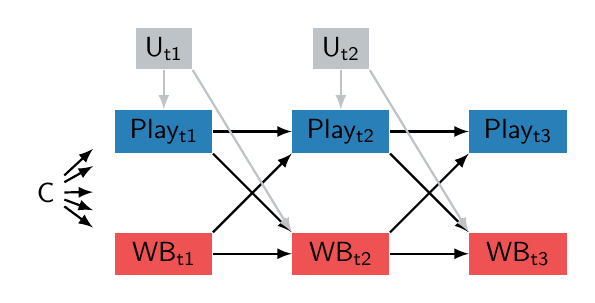
\begin{tikzpicture}
    % X
    \node[Node, fill=xFill] (x1) {Play\textsubscript{t1}};
    \node[Node, right =of x1, fill=xFill] (x2) {Play\textsubscript{t2}};
    \node[Node, right =of x2, fill=xFill] (x3) {Play\textsubscript{t3}};
    \draw[Arrow, thick] (x1.east) -- (x2.west);
    \draw[Arrow, thick] (x2.east) -- (x3.west);

    % Y
    \node[Node, below = of x1, fill=yFill] (y1){WB\textsubscript{t1}};
    \node[Node, right =of y1, fill=yFill] (y2) {WB\textsubscript{t2}};
    \node[Node, right =of y2, fill=yFill] (y3) {WB\textsubscript{t3}};
    \draw[Arrow, thick] (y1.east) -- (y2.west);
    \draw[Arrow, thick] (y2.east) -- (y3.west);

    % cross-lagged arrows
    \draw[Arrow, thick] (y1.north east) -- (x2.south west);
    \draw[Arrow, thick] (y2.north east) -- (x3.south west);
    \draw[Arrow, thick] (x1.south east) -- (y2.north west);
    \draw[Arrow, thick] (x2.south east) -- (y3.north west);

    % Time-invariant confounding
    \node[xshift=-1.5cm] (C) at ($(x1)!0.5!(y1)$) {C};
    \draw[Arrow, thick] (C) -- (-0.9, -0.22);
    \draw[Arrow, thick] (C) -- (-0.9, -0.44);
    \draw[Arrow, thick] (C) -- (-0.9, -0.77);
    \draw[Arrow, thick] (C) -- (-0.9, -1);
    \draw[Arrow, thick] (C) -- (-0.9, -1.22);

    % time-varying confounder
    % U1
    \node[above = 0.5 of x1, fill=tvFill] (U1){U\textsubscript{t1}};
    \draw[Arrow=tvFill, thick, color = tvFill] (U1.south) -- (x1.north);
    \draw[Arrow=tvFill, thick, color = tvFill] (U1.south east) -- (y2.north west);
    % U2
    \node[above = 0.5 of x2, fill=tvFill] (U2){U\textsubscript{t2}};
    \draw[Arrow=tvFill, thick, color = tvFill] (U2.south) -- (x2.north);
    \draw[Arrow=tvFill, thick, color = tvFill] (U2.south east) -- (y3.north west);
    \end{tikzpicture}
\end{adjustbox}
\end{document}
